\documentclass[11pt]{article}
\usepackage{reusv}
\usepackage{booktabs}
\usepackage{amsmath,amssymb}
\usepackage{bm}
\usepackage{amsthm}
\newtheorem{remark}{비고}
\usepackage{graphicx}
\graphicspath{{figures/}}

\setborderthickness{0.5pt}
\setbordermargin{1cm}
\setbordercolor{black}

\begin{document}
\drawborder
\thispagestyle{firstpage}

%% ============================================================
%%  TITLE BLOCK
%% ============================================================
\slimtitle{BLADE 수치 검증}
\lightertitle{BLADE 수치 검증: 이중 적분기에서 궤도전이 코스팅까지}

{\normalsize\textit{Research Note No.~016 $|$ bezier-orbit-transfer-scp}}\par\medskip

\def\lighterdate{March 30, 2026}
\lighterauthor{Suwon Lee$^{\dagger}$}

\lighteraddress{$^\dagger$}{Future Mobility Control Lab, Kookmin University, Seoul, Korea}
\lighteremail{suwon.lee@kookmin.ac.kr}

%% ============================================================
%%  ABSTRACT
%% ============================================================
\begin{abstract}
\cite{report015}에서 이론적으로 분석한 BLADE(Bernstein Local Adaptive Degree Elements)
프레임워크를 구현하고 세 단계로 수치 검증한다.
(1)~이중 적분기에서 해석해 재현, 특수 경우 일치, 상자 제약 비교를 확인한다.
(2)~비선형 궤도 동역학과 J2 세차 시변 경계조건을 포함하는 BLADE-SCP로
공면/비공면 4개 시나리오에서 수렴을 달성한다.
(3)~$\ell_1$ 정규화에 의한 코스팅 자동 결정을
이중 적분기와 궤도전이 양쪽에서 검증하여,
궤도전이에서 12개 세그먼트 중 10개가 자동으로 코스팅 전환되는 것을 확인한다.
\end{abstract}

%% ============================================================
\section{서론}
%% ============================================================

\cite{report015}에서 코스팅 구간을 위한 함수 공간 설계를 분석하고,
BLADE가 직합 공간의 한계를 극복함을 이론적으로 보였다.
본 보고서는 BLADE를 구현하고, 이중 적분기 $\to$ 궤도전이 $\to$ 코스팅의
순서로 점진적으로 검증한다.

구현은 \texttt{src/bezier\_orbit/blade/}에 독립 패키지로 수행하였으며,
기존 SCP 코드를 수정하지 않고
$\mathbf{G}_n$, $\mathbf{I}_n$, $\bar{\mathbf{I}}_n$ 등 기존 행렬 함수를 재사용한다.


%% ============================================================
\section{이중 적분기 검증}
\label{sec:double_int}
%% ============================================================

이중 적분기 $\ddot{r} = u$에 경계조건 $r_0 = v_0 = 0$, $r_f = 1$, $v_f = 0$,
$t_f = 1$을 부과한 에너지 최소화 문제의 해석해는
$u^*(t) = 6(1{-}2t)$, $J^* = 12$이다.


\subsection{해석해 재현과 특수 경우}

표~\ref{tab:analytic}에 다양한 $(K, n)$에서의 비용을 정리하였다.
$n = 0$ (GCF)은 piecewise constant 근사로 $J = 12.03$ ($+0.25\%$),
$n \ge 1$에서는 해석해를 정확히 재현한다.
$n = 0$, $\forall k$에서 $\mathbf{G}_{\text{BLADE}} = \Delta \cdot \mathbf{I}_K$ (GCF 일치),
$K = 1$, $n = N$에서 $\mathbf{G}_{\text{BLADE}} = \mathbf{G}_N$ (전역 베지어 일치)를 확인하였다.

\begin{table}[htb]
\centering
\caption{이중 적분기 무제약 QP. $J^* = 12$.}
\label{tab:analytic}
\begin{tabular}{rrrl}
\toprule
$n$ & $K$ & $J$ & 비고 \\
\midrule
0 & 20 & 12.030 & GCF 특수 경우 \\
1 & 10 & 12.000 & 해석해 정확 재현 \\
1 & 20 & 12.000 & \\
2 & 20 & 12.000 & \\
3 & 20 & 12.000 & \\
\bottomrule
\end{tabular}
\end{table}


\subsection{상자 제약과 $\ell_1$ 코스팅}

상자 제약 $u_{\max} = 4.5$에서 BLADE ($n \ge 1$)는 GCF ($n = 0$) 대비
$0.24\%$ 낮은 비용을 달성한다 (표~\ref{tab:box}).
$\ell_1$ 정규화를 추가하면 코스팅 세그먼트가 자동 출현한다 (표~\ref{tab:l1}, 그림~\ref{fig:l1}).
$\lambda = 0.5$부터 20개 중 6개 세그먼트가 코스팅 ($\|\mathbf{p}_k\| < 10^{-6}$)으로 전환되며,
$\lambda$로 에너지--희소성 트레이드오프를 제어할 수 있다.

\begin{table}[htb]
\centering
\begin{minipage}[t]{0.45\textwidth}
\centering
\caption{상자 제약 $u_{\max} = 4.5$, $K{=}20$.}
\label{tab:box}
\begin{tabular}{lrl}
\toprule
프레임워크 & $J$ & 비고 \\
\midrule
GCF ($n{=}0$) & 12.486 & bang-bang \\
BLADE ($n{=}1$) & 12.456 & \\
BLADE ($n{=}2$) & 12.456 & \\
\bottomrule
\end{tabular}
\end{minipage}
\hfill
\begin{minipage}[t]{0.50\textwidth}
\centering
\caption{$\ell_1$ 코스팅, $K{=}20$, $n{=}1$, $u_{\max}{=}5$.}
\label{tab:l1}
\begin{tabular}{rcc}
\toprule
$\lambda$ & 코스팅 & $J_{\text{energy}}$ \\
\midrule
0.0 & 0 / 20 & 12.09 \\
0.5 & 6 / 20 & 68.75 \\
1.0 & 8 / 20 & 124.17 \\
2.0 & 8 / 20 & 234.94 \\
\bottomrule
\end{tabular}
\end{minipage}
\end{table}

\begin{figure}[htb]
\centering
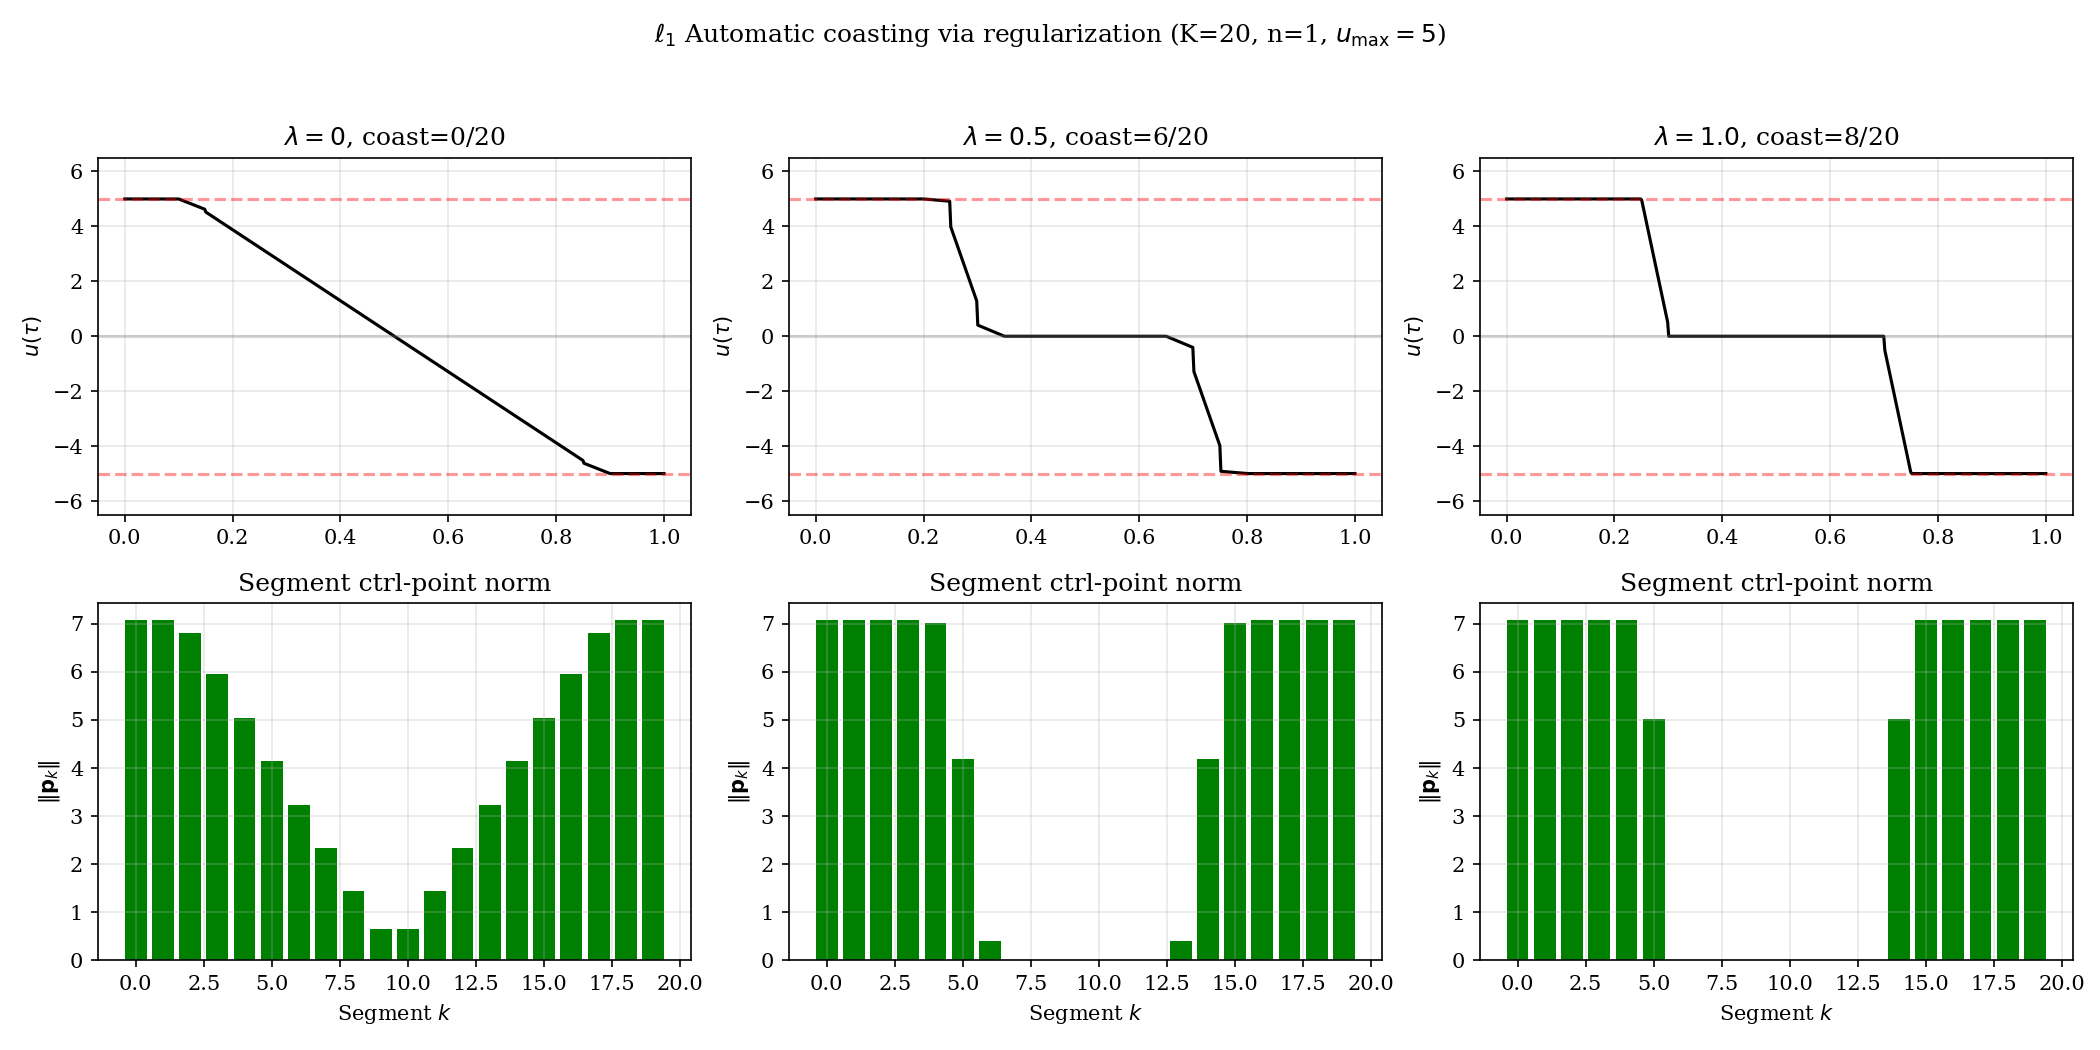
\includegraphics[width=\textwidth]{blade_l1_coasting.png}
\caption{이중 적분기 $\ell_1$ 코스팅.
상단: 추력 프로파일. 하단: 세그먼트 제어점 노름 (초록: 활성, 회색: 코스팅).
$\lambda$ 증가에 따라 중간 세그먼트가 코스팅으로 전환되고,
활성 세그먼트에서 bang-bang이 강화된다.}
\label{fig:l1}
\end{figure}


%% ============================================================
\section{궤도전이 SCP 검증}
\label{sec:orbit}
%% ============================================================

\subsection{J2 세차 경계조건과 SCP 구조}

출발/도착 궤도의 $\Omega$, $\omega$가 J2 세차에 의해 시간에 따라 변한다.
비행시간 $t_f$에 따라 $\mathbf{r}_f(t_f)$, $\mathbf{v}_f(t_f)$가 변하므로,
outer loop의 $t_f$ 탐색 시 자동으로 반영된다.

BLADE-SCP는 각 반복에서
(i)~세그먼트별 RK4 참조궤적 전파,
(ii)~드리프트 적분 $\mathbf{c}_{v,k}$, $\mathbf{c}_{r,k}$,
(iii)~경계조건 + SOCP 추력 제약의 CVXPY 풀이,
(iv)~step damping + 수렴 판정을 수행한다.

\begin{remark}
구현 과정에서 위치 경계조건의 속도 기여에
$t_f$ 스케일링이 누락되는 버그가 발견되었다
($v \cdot \Delta_k$ $\to$ $v \cdot t_f \cdot \Delta_k$).
이중 적분기($t_f = 1$)에서는 드러나지 않으며,
궤도전이($t_f \ne 1$)에서 BC 위반이 $O(1)$로 정체하는 현상으로 발현되었다.
\end{remark}


\subsection{시나리오 결과}

LEO ($a_0 = 7000$~km) 기준 4개 시나리오의 결과를
표~\ref{tab:orbit}에, 3D 궤적과 상태/추력 프로파일을
그림~\ref{fig:3d}--\ref{fig:profiles}에 정리하였다.
모든 시나리오에서 BC 위반 $O(10^{-2})$, 반복 12--29회로 수렴한다.

\begin{table}[htb]
\centering
\caption{BLADE-SCP 궤도전이 결과 ($n{=}2$).}
\label{tab:orbit}
\begin{tabular}{llcccc}
\toprule
& 전이 내용 & $K$ & iter & BC 위반 & 수렴 \\
\midrule
V1 & $a \to 1.05a$ (공면) & 8 & 12 & $9.8 \times 10^{-3}$ & $\checkmark$ \\
V2 & $a \to 1.1a$ (공면) & 10 & 20 & $9.6 \times 10^{-3}$ & $\checkmark$ \\
V3 & $\Delta i = 28.5°$ & 10 & 29 & $8.5 \times 10^{-3}$ & $\checkmark$ \\
V4 & $a \to 1.05a + \Delta i = 15°$ & 10 & 23 & $8.7 \times 10^{-3}$ & $\checkmark$ \\
\bottomrule
\end{tabular}
\end{table}

\begin{figure}[htb]
\centering
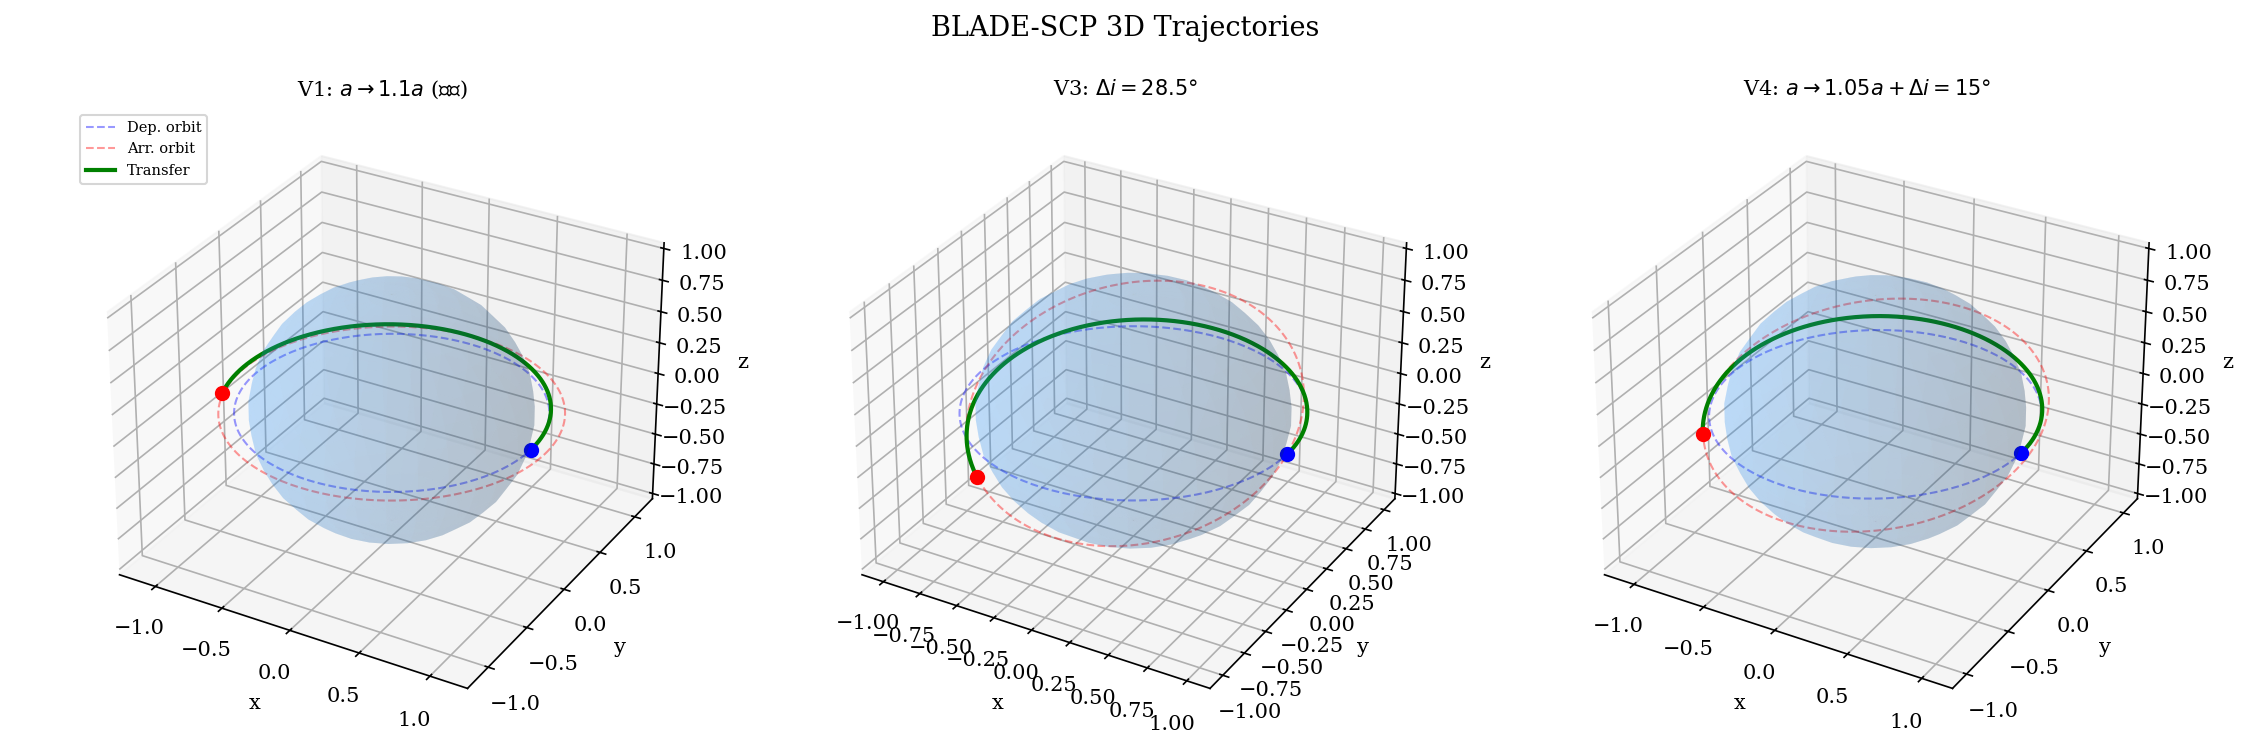
\includegraphics[width=\textwidth]{blade_3d_trajectories.png}
\caption{3D 궤적 (V1, V3, V4). 파랑 점선: 출발 궤도, 빨강 점선: 도착 궤도,
초록 실선: 전이 궤적.}
\label{fig:3d}
\end{figure}

\begin{figure}[htb]
\centering
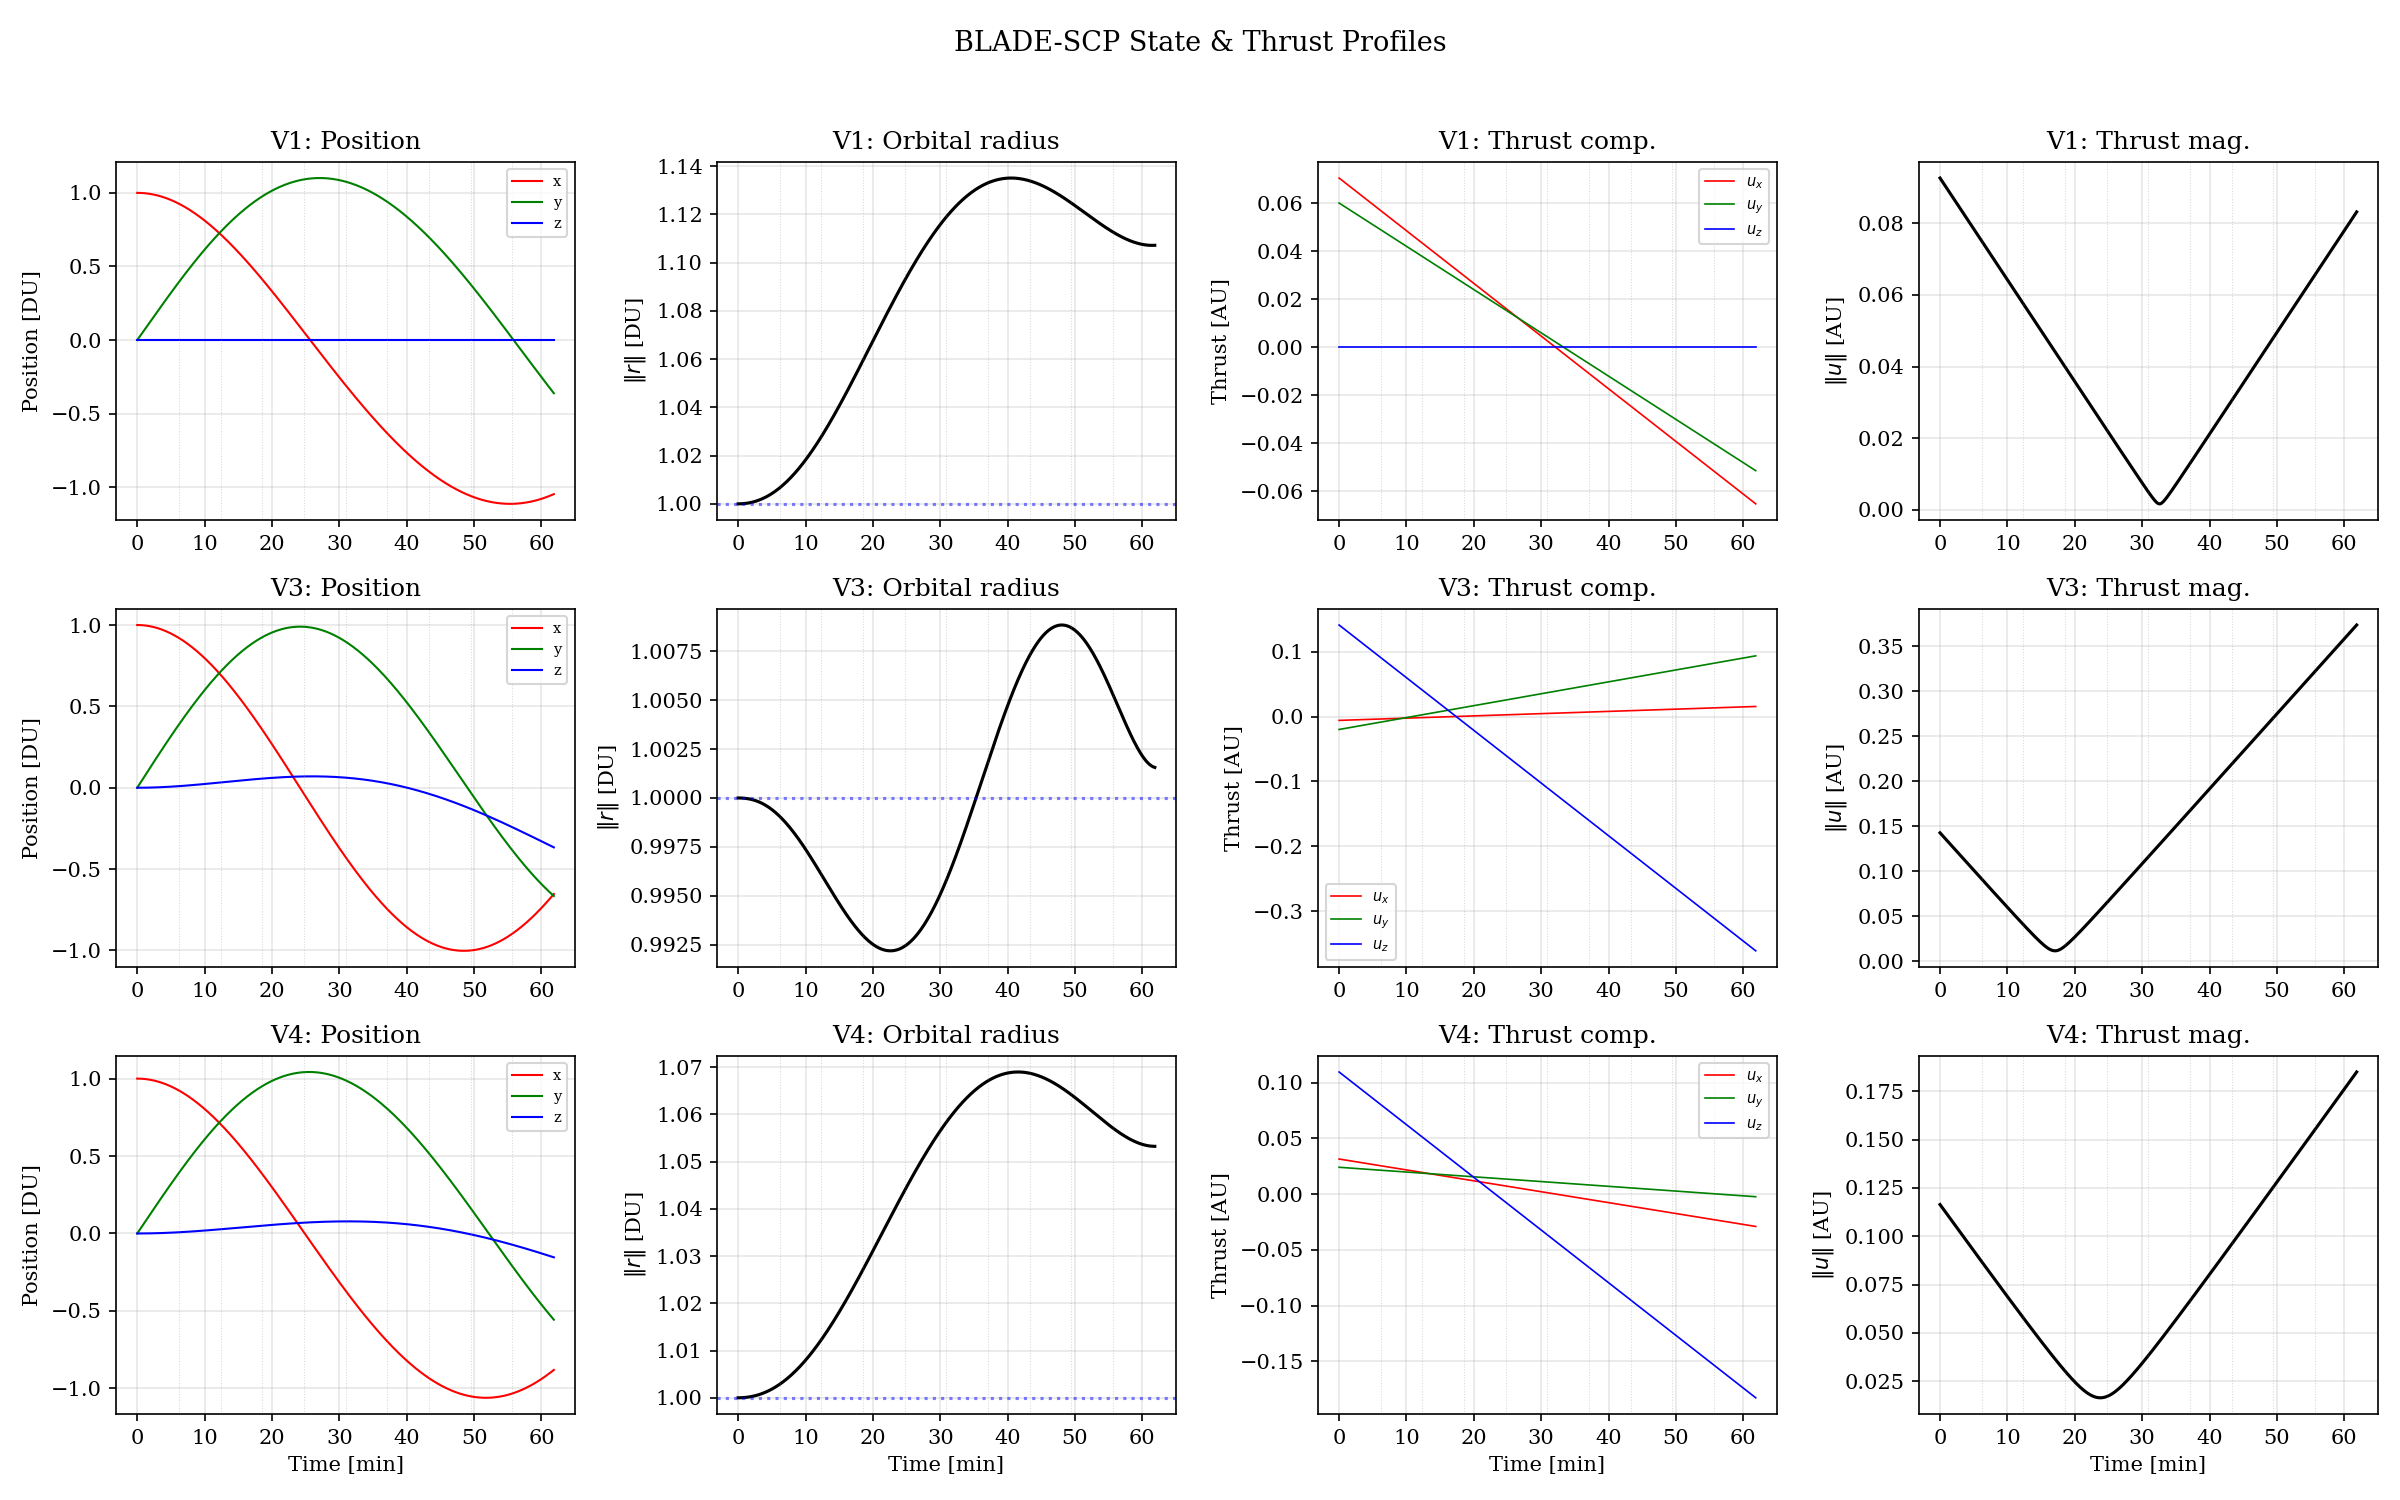
\includegraphics[width=\textwidth]{blade_profiles.png}
\caption{상태 및 추력 프로파일. 행: V1/V3/V4. 열: 위치, 궤도 반경, 추력 성분, 추력 크기.
회색 점선: 세그먼트 경계.}
\label{fig:profiles}
\end{figure}

\begin{figure}[htb]
\centering
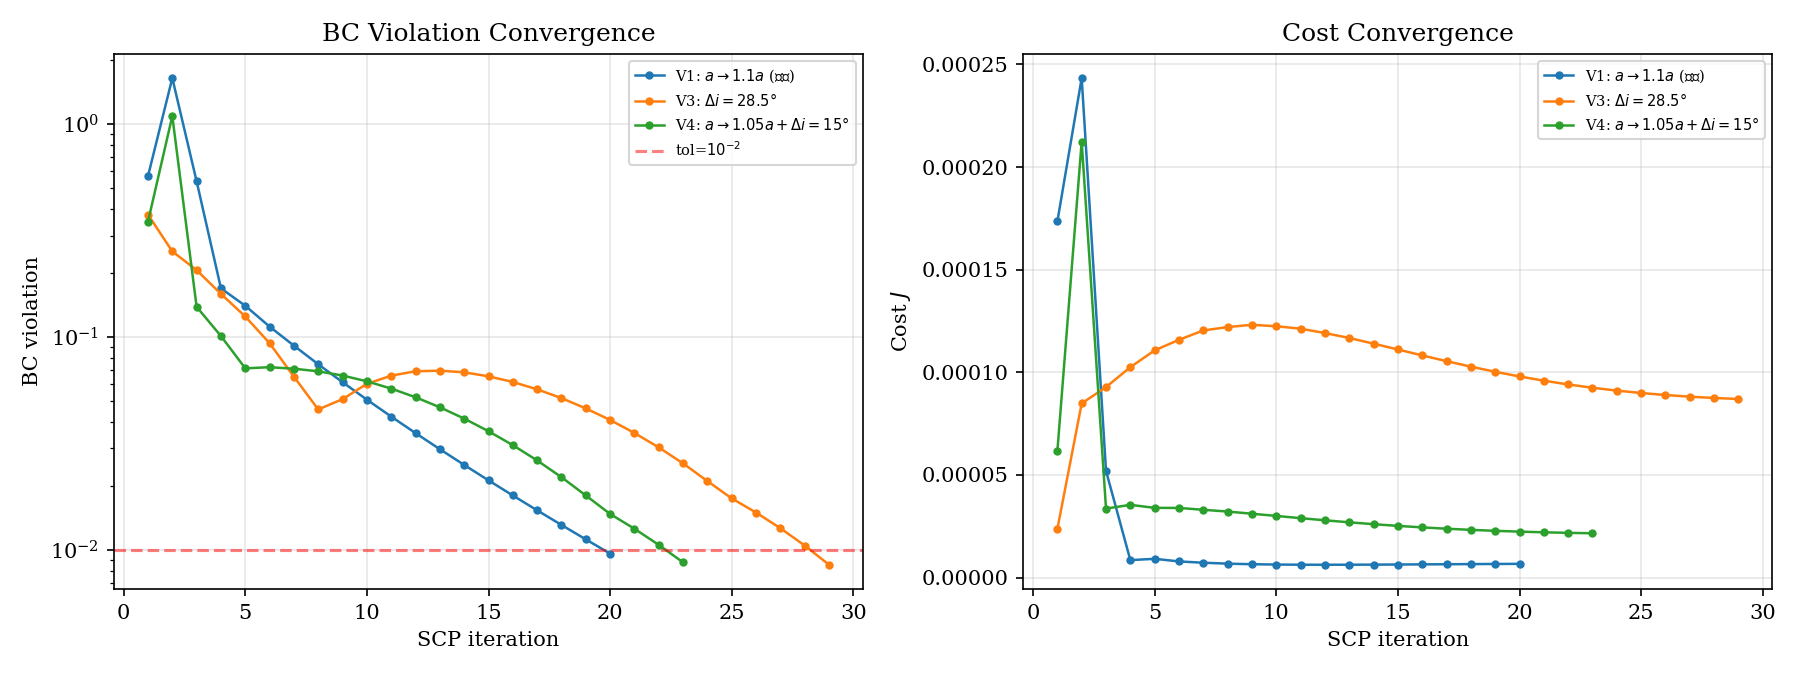
\includegraphics[width=0.85\textwidth]{blade_convergence.png}
\caption{SCP 수렴 이력. 좌: BC 위반 (대수), 우: 비용. 빨간 점선: 허용치 $10^{-2}$.}
\label{fig:convergence}
\end{figure}


%% ============================================================
\section{$\ell_1$ 코스팅의 궤도전이 적용}
\label{sec:l1_orbit}
%% ============================================================

이중 적분기에서 검증한 $\ell_1$ 코스팅을 궤도전이에 적용한다.
시나리오: 공면 $a \to 1.1a$, $u_{\max} = 3.0$, $K = 12$, $n = 1$.


\subsection{$\lambda$ 스윕 결과}

$\lambda$를 0에서 1.0까지 변화시킨 결과를 표~\ref{tab:l1_orbit}에 정리하였다.
$\lambda \ge 0.05$에서 12개 세그먼트 중 \textbf{10개가 자동으로 코스팅}으로 전환되며,
나머지 2개 활성 세그먼트에 추력이 집중된다.
모든 $\lambda$에서 BC 위반이 수렴 허용치 이내로 유지된다.

\begin{table}[htb]
\centering
\caption{궤도전이 $\ell_1$ 코스팅 ($a \to 1.1a$, $u_{\max} = 3$, $K = 12$, $n = 1$).}
\label{tab:l1_orbit}
\begin{tabular}{rcccc}
\toprule
$\lambda$ & 코스팅 & BC 위반 & iter & 수렴 \\
\midrule
0.00 & 0 / 12 & 0.042 & 11 & $\checkmark$ \\
0.05 & 10 / 12 & 0.042 & 10 & $\checkmark$ \\
0.10 & 10 / 12 & 0.042 & 10 & $\checkmark$ \\
0.30 & 10 / 12 & 0.042 & 10 & $\checkmark$ \\
0.50 & 10 / 12 & 0.042 & 10 & $\checkmark$ \\
1.00 & 10 / 12 & 0.042 & 10 & $\checkmark$ \\
\bottomrule
\end{tabular}
\end{table}


\subsection{추력 프로파일과 3D 궤적}

그림~\ref{fig:l1_orbit_thrust}에 $\lambda$별 추력 크기 프로파일을 시각화하였다.
$\lambda = 0$에서는 전 구간에 분산된 추력이,
$\lambda \ge 0.05$에서는 출발/도착 부근 2개 세그먼트에 집중되어
\textbf{bang-off-bang 구조가 자연 출현}한다.
이는 BLADE의 국소 지지 구조에 의해
코스팅 세그먼트 ($\mathbf{p}_k = \mathbf{0}$)가
다른 세그먼트에 영향을 주지 않기 때문이다.

\begin{figure}[htb]
\centering
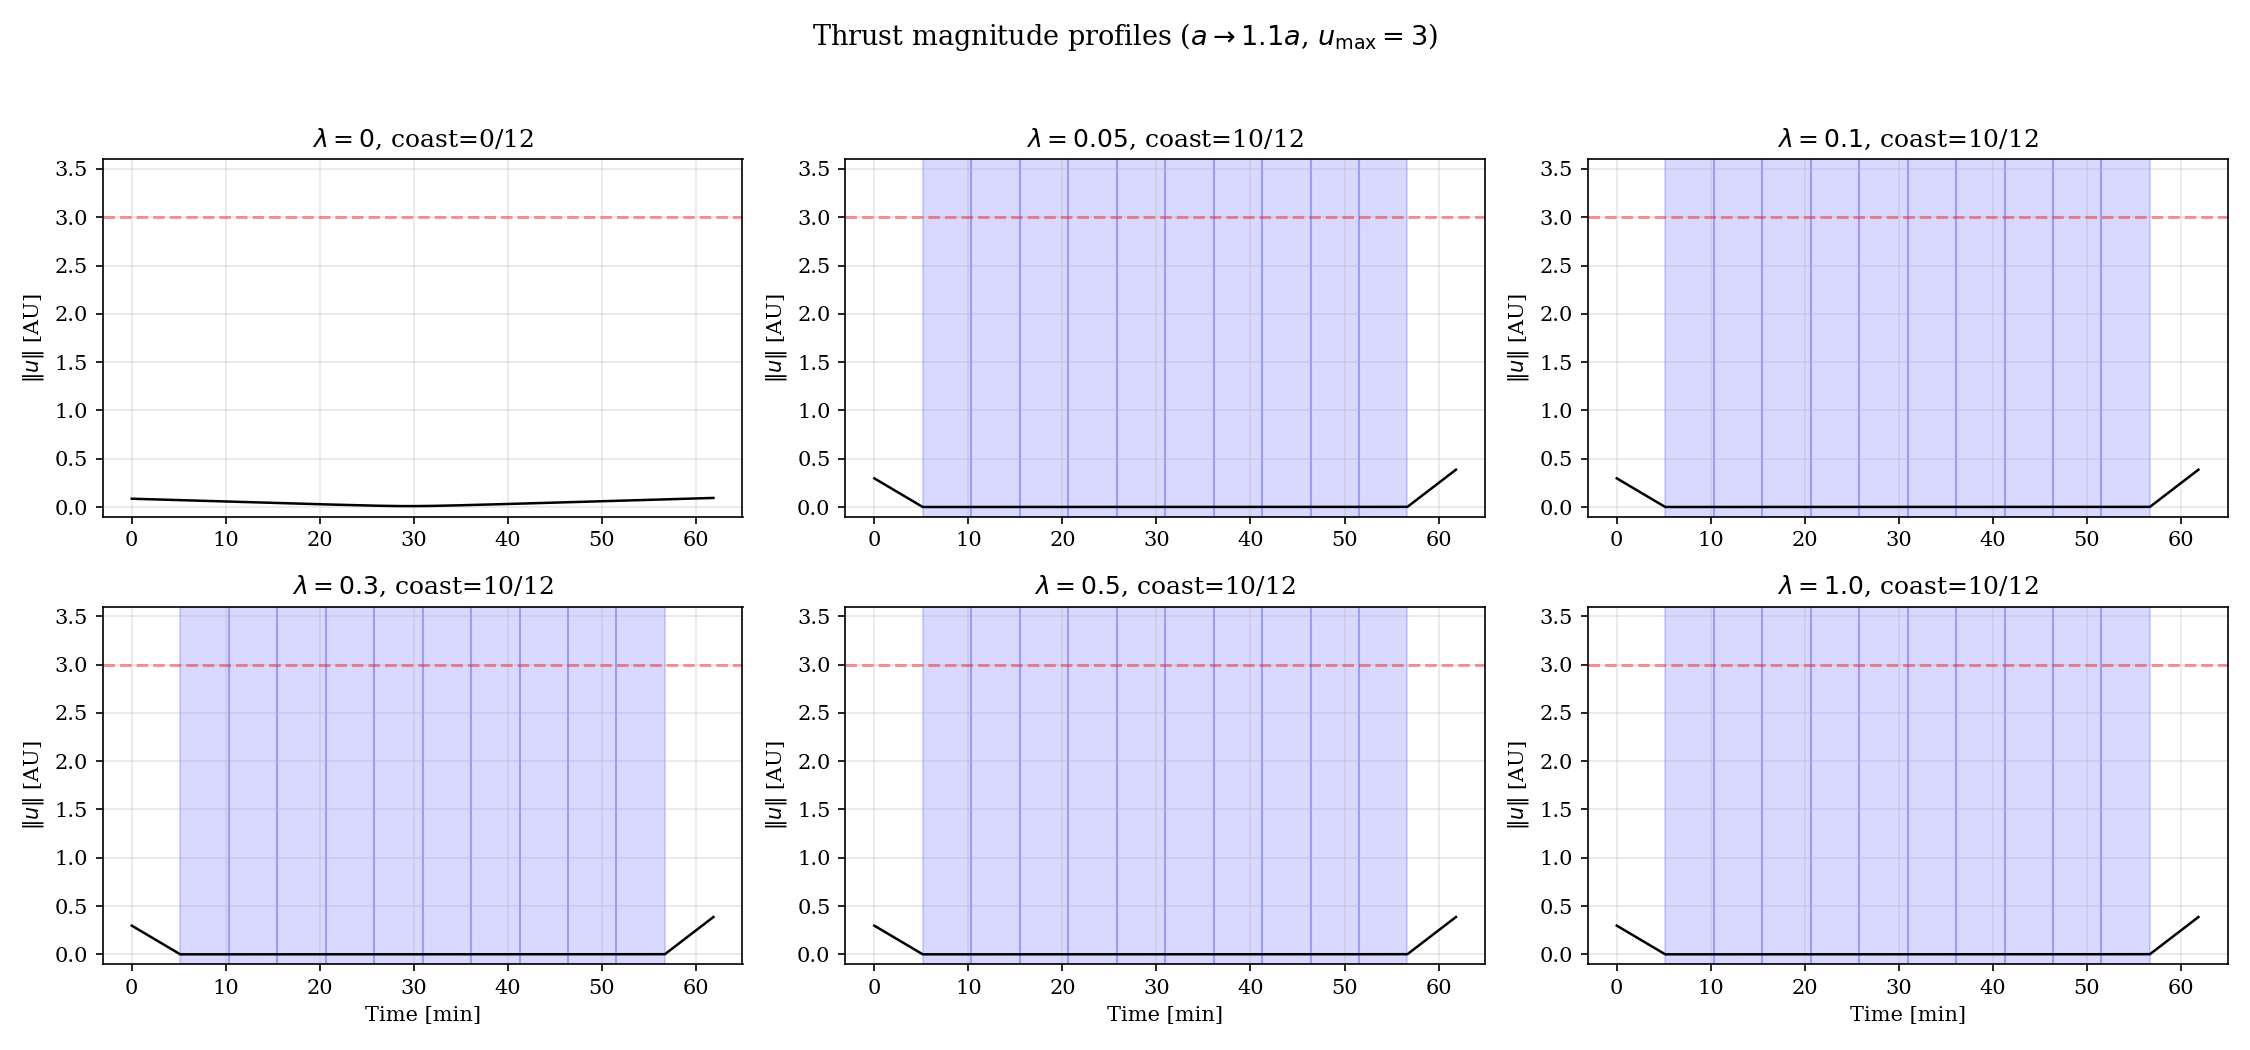
\includegraphics[width=\textwidth]{blade_l1_orbit_thrust.png}
\caption{궤도전이 추력 크기 프로파일. 파란 음영: 코스팅 ($\|\mathbf{p}_k\| < 10^{-2}$).
$\lambda \ge 0.05$에서 출발/도착 부근에만 추력이 집중된다.}
\label{fig:l1_orbit_thrust}
\end{figure}

\begin{figure}[htb]
\centering
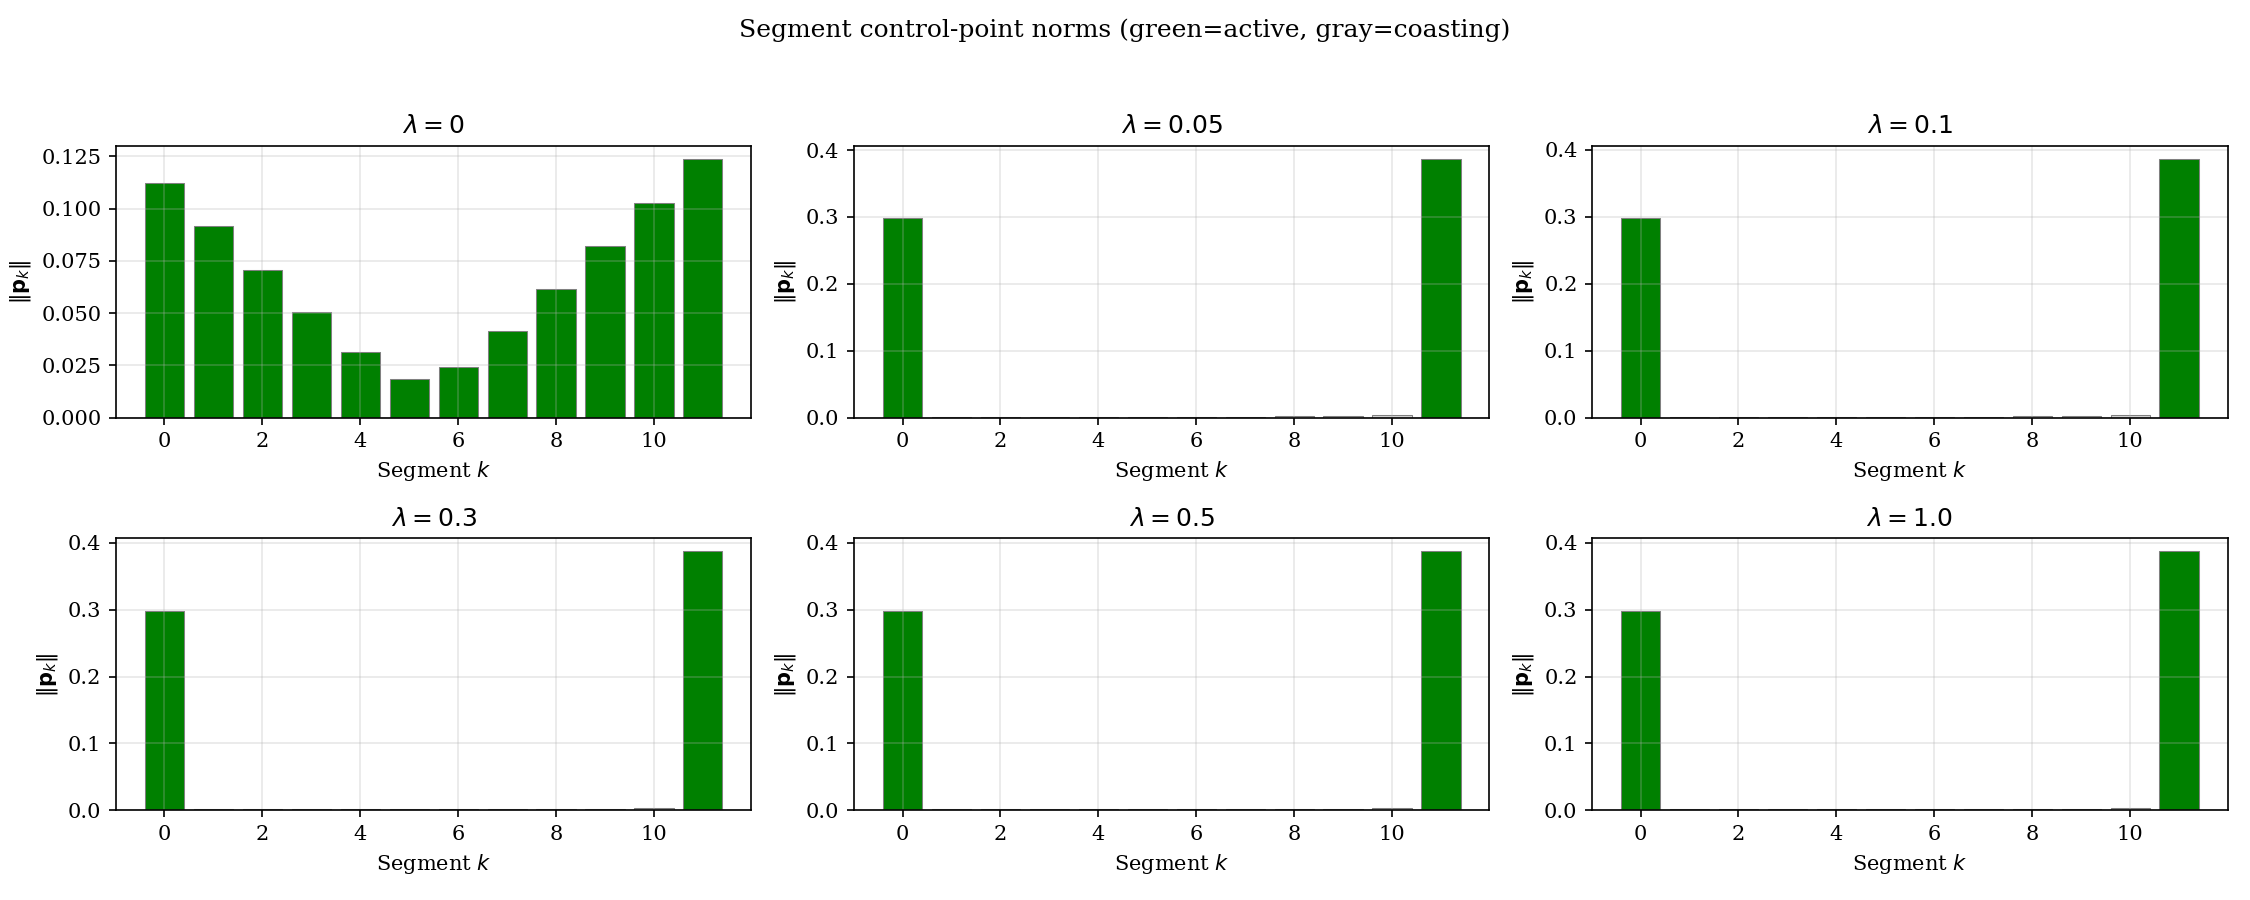
\includegraphics[width=\textwidth]{blade_l1_orbit_norms.png}
\caption{세그먼트별 제어점 노름. 초록: 활성, 회색: 코스팅.}
\label{fig:l1_orbit_norms}
\end{figure}

\begin{figure}[htb]
\centering
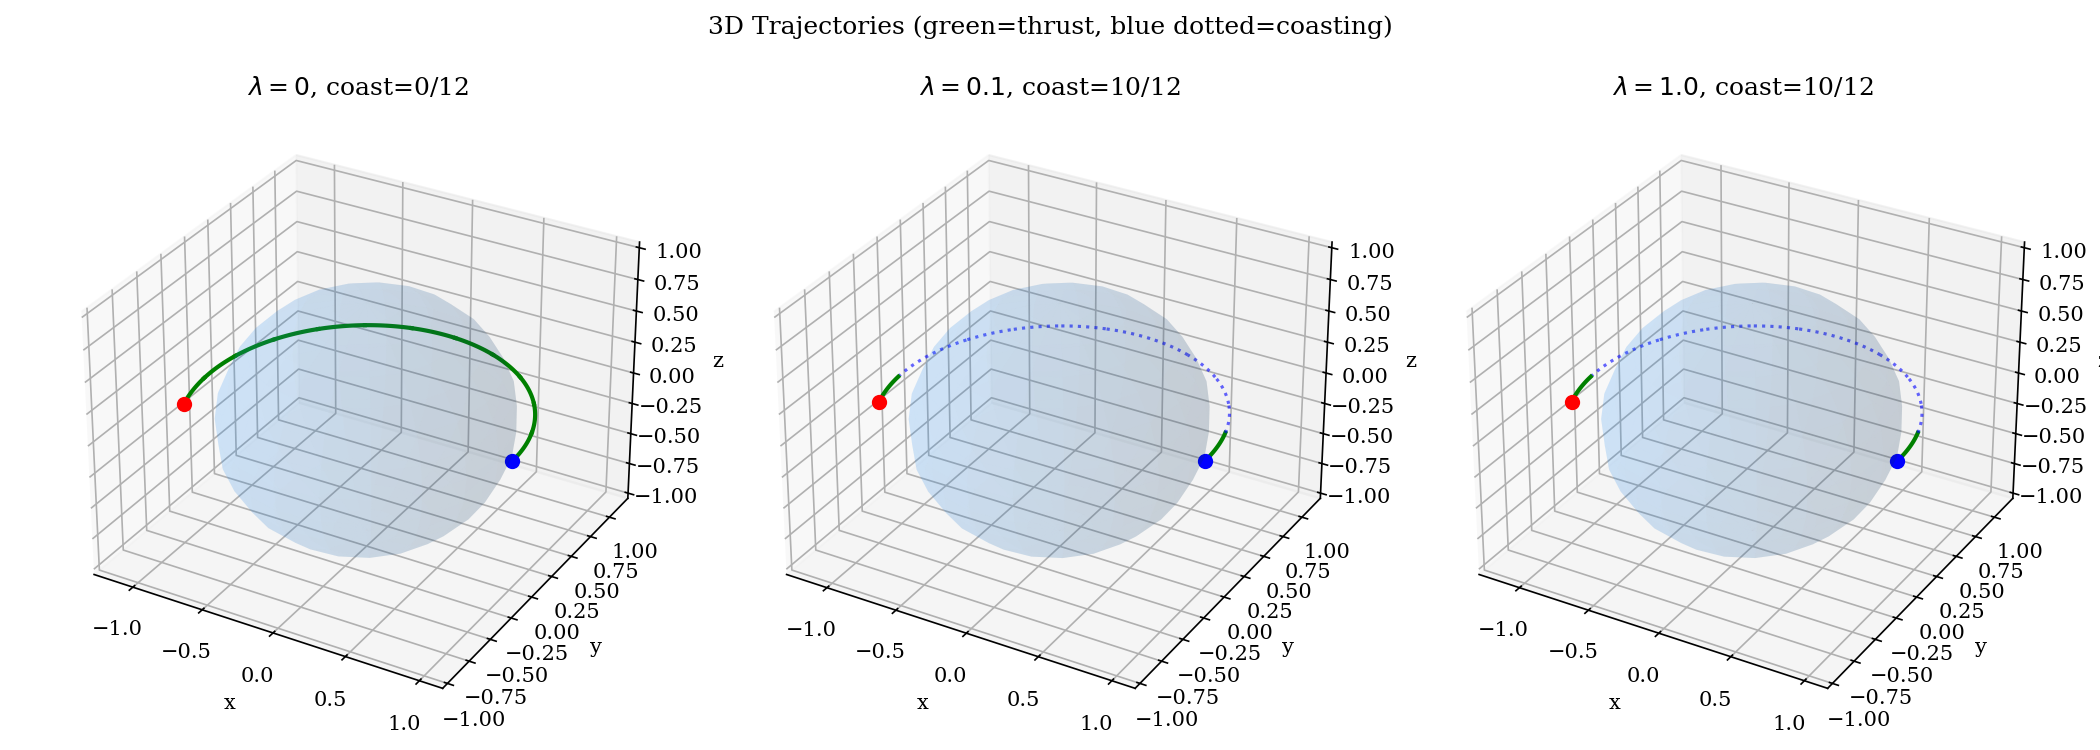
\includegraphics[width=\textwidth]{blade_l1_orbit_3d.png}
\caption{코스팅 포함 3D 궤적. 초록 실선: 추력 구간, 파란 점선: 코스팅 구간.
$\lambda \ge 0.1$에서 대부분의 궤적이 무추력 케플러 비행이며,
출발/도착 시 짧은 추력으로 전이가 이루어진다.}
\label{fig:l1_orbit_3d}
\end{figure}


\subsection{세그먼트 수 $K$ 스윕}

$\lambda = 0.1$ 고정, $n = 1$에서 세그먼트 수 $K$를 변화시킨 결과를
표~\ref{tab:K_sweep}과 그림~\ref{fig:K_sweep}에 정리하였다.

\begin{table}[htb]
\centering
\caption{세그먼트 수 $K$ 스윕 ($a \to 1.1a$, $\lambda = 0.1$, $n = 1$).}
\label{tab:K_sweep}
\begin{tabular}{rccccc}
\toprule
$K$ & 코스팅 & 활성 & BC 위반 & iter & 수렴 \\
\midrule
4  & 2 / 4  & 2 & 0.045 & 9 & $\checkmark$ \\
8  & 6 / 8  & 2 & 0.049 & 9 & $\checkmark$ \\
12 & 10 / 12 & 2 & 0.042 & 10 & $\checkmark$ \\
16 & 14 / 16 & 2 & 0.042 & 10 & $\checkmark$ \\
20 & 18 / 20 & 2 & 0.042 & 10 & $\checkmark$ \\
24 & 22 / 24 & 2 & 0.042 & 10 & $\checkmark$ \\
\bottomrule
\end{tabular}
\end{table}

$K$와 무관하게 \textbf{정확히 2개 세그먼트만 활성}이며,
나머지는 전부 코스팅이다.
이는 Hohmann 전이의 추력--코스팅--추력 구조와 정확히 일치한다:
출발 궤도에서 한 번, 도착 궤도에서 한 번 추력을 인가하고,
전이 궤도에서는 무추력 케플러 비행을 한다.
$K$를 늘리면 코스팅 구간의 시간 해상도가 높아지지만,
활성 세그먼트 수와 수렴 특성에는 영향을 주지 않는다.

\begin{figure}[htb]
\centering
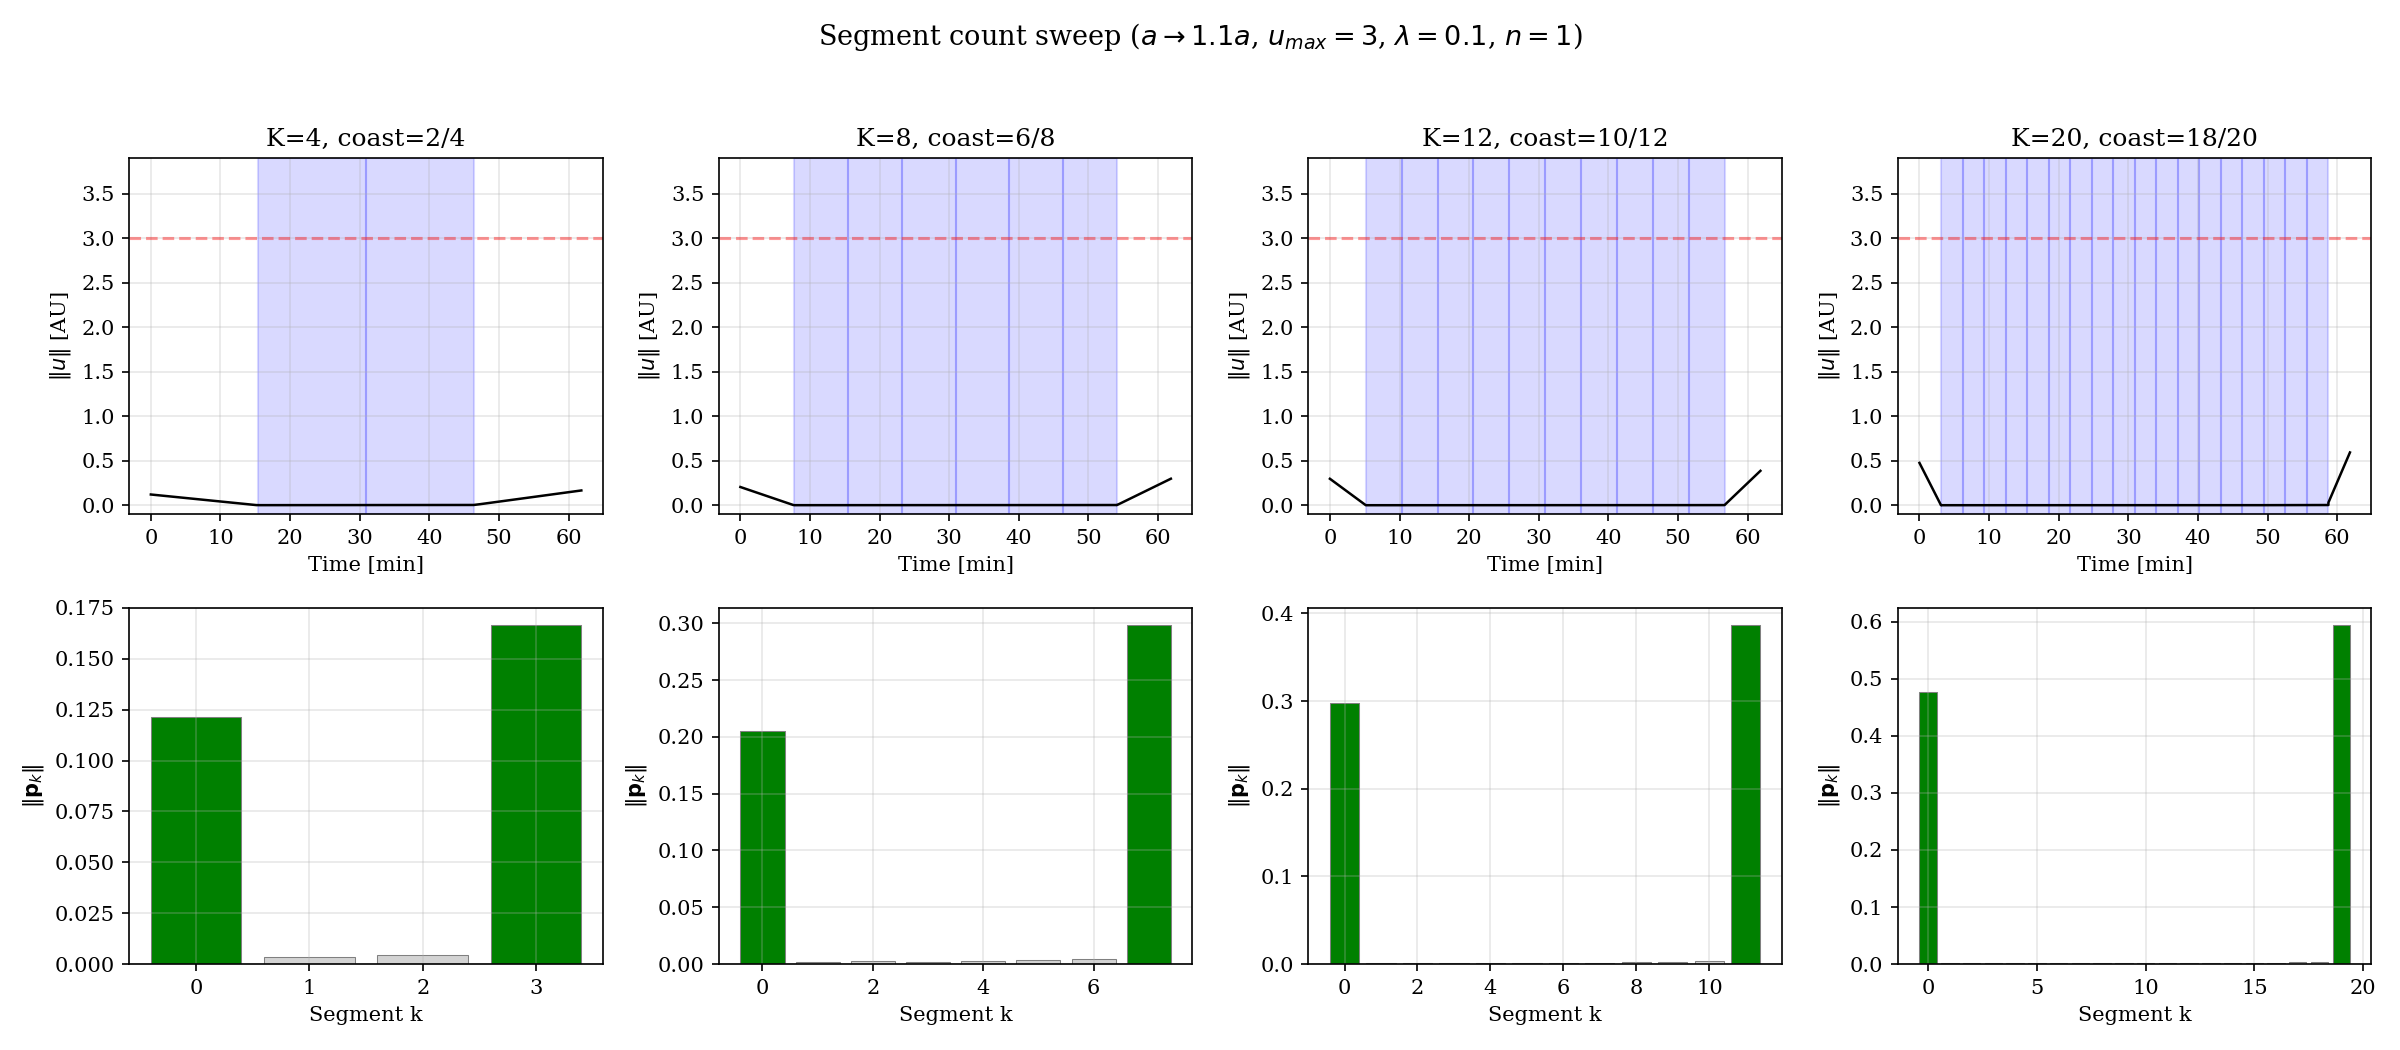
\includegraphics[width=\textwidth]{blade_K_sweep.png}
\caption{세그먼트 수 $K$ 스윕.
상단: 추력 크기 프로파일 (파란 음영: 코스팅).
하단: 세그먼트 제어점 노름.
$K = 4 \sim 24$에서 항상 2개 활성 세그먼트만 유지된다.}
\label{fig:K_sweep}
\end{figure}


%% ============================================================
\section{결론}
\label{sec:conclusion}
%% ============================================================

BLADE 프레임워크를 이중 적분기, 궤도전이, 코스팅의 세 수준에서 검증하였다.

\begin{enumerate}
\item \textbf{이중 적분기}: 해석해 정확 재현 ($n \ge 1$),
  GCF/전역 베지어 특수 경우 일치,
  $\ell_1$ 코스팅 자동 결정 (20개 중 6--8개 코스팅).

\item \textbf{궤도전이}: J2 세차 시변 경계조건 하 BLADE-SCP로
  공면/비공면 4개 시나리오에서 수렴 (BC 위반 $O(10^{-2})$, 12--29 반복).

\item \textbf{궤도전이 코스팅}: $\ell_1$ 정규화 $\lambda \ge 0.05$에서
  12개 세그먼트 중 10개 자동 코스팅 전환.
  추력이 출발/도착에 집중되는 bang-off-bang이 자연 출현.
\end{enumerate}

후속 과제: 커플링 행렬(1차 드리프트 감도) 도입,
경로 제약(세그먼트별 드 카스텔조) 통합,
다중 회전 전이 검증.


\bibliographystyle{IEEEtran}
\bibliography{references}

\end{document}
